% Options for packages loaded elsewhere
\PassOptionsToPackage{unicode}{hyperref}
\PassOptionsToPackage{hyphens}{url}
%
\documentclass[
]{article}
\usepackage{amsmath,amssymb}
\usepackage{iftex}
\ifPDFTeX
  \usepackage[T1]{fontenc}
  \usepackage[utf8]{inputenc}
  \usepackage{textcomp} % provide euro and other symbols
\else % if luatex or xetex
  \usepackage{unicode-math} % this also loads fontspec
  \defaultfontfeatures{Scale=MatchLowercase}
  \defaultfontfeatures[\rmfamily]{Ligatures=TeX,Scale=1}
\fi
\usepackage{lmodern}
\ifPDFTeX\else
  % xetex/luatex font selection
\fi
% Use upquote if available, for straight quotes in verbatim environments
\IfFileExists{upquote.sty}{\usepackage{upquote}}{}
\IfFileExists{microtype.sty}{% use microtype if available
  \usepackage[]{microtype}
  \UseMicrotypeSet[protrusion]{basicmath} % disable protrusion for tt fonts
}{}
\makeatletter
\@ifundefined{KOMAClassName}{% if non-KOMA class
  \IfFileExists{parskip.sty}{%
    \usepackage{parskip}
  }{% else
    \setlength{\parindent}{0pt}
    \setlength{\parskip}{6pt plus 2pt minus 1pt}}
}{% if KOMA class
  \KOMAoptions{parskip=half}}
\makeatother
\usepackage{xcolor}
\usepackage[margin=1in]{geometry}
\usepackage{color}
\usepackage{fancyvrb}
\newcommand{\VerbBar}{|}
\newcommand{\VERB}{\Verb[commandchars=\\\{\}]}
\DefineVerbatimEnvironment{Highlighting}{Verbatim}{commandchars=\\\{\}}
% Add ',fontsize=\small' for more characters per line
\usepackage{framed}
\definecolor{shadecolor}{RGB}{248,248,248}
\newenvironment{Shaded}{\begin{snugshade}}{\end{snugshade}}
\newcommand{\AlertTok}[1]{\textcolor[rgb]{0.94,0.16,0.16}{#1}}
\newcommand{\AnnotationTok}[1]{\textcolor[rgb]{0.56,0.35,0.01}{\textbf{\textit{#1}}}}
\newcommand{\AttributeTok}[1]{\textcolor[rgb]{0.13,0.29,0.53}{#1}}
\newcommand{\BaseNTok}[1]{\textcolor[rgb]{0.00,0.00,0.81}{#1}}
\newcommand{\BuiltInTok}[1]{#1}
\newcommand{\CharTok}[1]{\textcolor[rgb]{0.31,0.60,0.02}{#1}}
\newcommand{\CommentTok}[1]{\textcolor[rgb]{0.56,0.35,0.01}{\textit{#1}}}
\newcommand{\CommentVarTok}[1]{\textcolor[rgb]{0.56,0.35,0.01}{\textbf{\textit{#1}}}}
\newcommand{\ConstantTok}[1]{\textcolor[rgb]{0.56,0.35,0.01}{#1}}
\newcommand{\ControlFlowTok}[1]{\textcolor[rgb]{0.13,0.29,0.53}{\textbf{#1}}}
\newcommand{\DataTypeTok}[1]{\textcolor[rgb]{0.13,0.29,0.53}{#1}}
\newcommand{\DecValTok}[1]{\textcolor[rgb]{0.00,0.00,0.81}{#1}}
\newcommand{\DocumentationTok}[1]{\textcolor[rgb]{0.56,0.35,0.01}{\textbf{\textit{#1}}}}
\newcommand{\ErrorTok}[1]{\textcolor[rgb]{0.64,0.00,0.00}{\textbf{#1}}}
\newcommand{\ExtensionTok}[1]{#1}
\newcommand{\FloatTok}[1]{\textcolor[rgb]{0.00,0.00,0.81}{#1}}
\newcommand{\FunctionTok}[1]{\textcolor[rgb]{0.13,0.29,0.53}{\textbf{#1}}}
\newcommand{\ImportTok}[1]{#1}
\newcommand{\InformationTok}[1]{\textcolor[rgb]{0.56,0.35,0.01}{\textbf{\textit{#1}}}}
\newcommand{\KeywordTok}[1]{\textcolor[rgb]{0.13,0.29,0.53}{\textbf{#1}}}
\newcommand{\NormalTok}[1]{#1}
\newcommand{\OperatorTok}[1]{\textcolor[rgb]{0.81,0.36,0.00}{\textbf{#1}}}
\newcommand{\OtherTok}[1]{\textcolor[rgb]{0.56,0.35,0.01}{#1}}
\newcommand{\PreprocessorTok}[1]{\textcolor[rgb]{0.56,0.35,0.01}{\textit{#1}}}
\newcommand{\RegionMarkerTok}[1]{#1}
\newcommand{\SpecialCharTok}[1]{\textcolor[rgb]{0.81,0.36,0.00}{\textbf{#1}}}
\newcommand{\SpecialStringTok}[1]{\textcolor[rgb]{0.31,0.60,0.02}{#1}}
\newcommand{\StringTok}[1]{\textcolor[rgb]{0.31,0.60,0.02}{#1}}
\newcommand{\VariableTok}[1]{\textcolor[rgb]{0.00,0.00,0.00}{#1}}
\newcommand{\VerbatimStringTok}[1]{\textcolor[rgb]{0.31,0.60,0.02}{#1}}
\newcommand{\WarningTok}[1]{\textcolor[rgb]{0.56,0.35,0.01}{\textbf{\textit{#1}}}}
\usepackage{graphicx}
\makeatletter
\def\maxwidth{\ifdim\Gin@nat@width>\linewidth\linewidth\else\Gin@nat@width\fi}
\def\maxheight{\ifdim\Gin@nat@height>\textheight\textheight\else\Gin@nat@height\fi}
\makeatother
% Scale images if necessary, so that they will not overflow the page
% margins by default, and it is still possible to overwrite the defaults
% using explicit options in \includegraphics[width, height, ...]{}
\setkeys{Gin}{width=\maxwidth,height=\maxheight,keepaspectratio}
% Set default figure placement to htbp
\makeatletter
\def\fps@figure{htbp}
\makeatother
\setlength{\emergencystretch}{3em} % prevent overfull lines
\providecommand{\tightlist}{%
  \setlength{\itemsep}{0pt}\setlength{\parskip}{0pt}}
\setcounter{secnumdepth}{-\maxdimen} % remove section numbering
\ifLuaTeX
  \usepackage{selnolig}  % disable illegal ligatures
\fi
\IfFileExists{bookmark.sty}{\usepackage{bookmark}}{\usepackage{hyperref}}
\IfFileExists{xurl.sty}{\usepackage{xurl}}{} % add URL line breaks if available
\urlstyle{same}
\hypersetup{
  pdftitle={Life\_Table},
  pdfauthor={Zhuodiao Kuang},
  hidelinks,
  pdfcreator={LaTeX via pandoc}}

\title{Life\_Table}
\author{Zhuodiao Kuang}
\date{2023-09-29}

\begin{document}
\maketitle

\hypertarget{load-packages}{%
\section{Load packages}\label{load-packages}}

\begin{Shaded}
\begin{Highlighting}[]
\FunctionTok{library}\NormalTok{(survival)}
\FunctionTok{library}\NormalTok{(tidyverse)}
\FunctionTok{library}\NormalTok{(ggfortify)}
\FunctionTok{library}\NormalTok{(dplyr)}
\FunctionTok{library}\NormalTok{(ggplot2)}
\FunctionTok{library}\NormalTok{(biostat3)}
\FunctionTok{library}\NormalTok{(knitr)}
\end{Highlighting}
\end{Shaded}

\hypertarget{ovarian-cancer}{%
\section{Ovarian Cancer:}\label{ovarian-cancer}}

\begin{itemize}
\tightlist
\item
  futime: survival or censoring time(day)
\item
  fustat: censoring status(censor = 0)
\item
  age: in years
\item
  resid.ds: residual disease present(1=no, 2=yes)
\item
  rx: treatment group
\item
  ecog.ps: ECOG performance status(1 is better)
\end{itemize}

\begin{Shaded}
\begin{Highlighting}[]
\FunctionTok{data}\NormalTok{(}\StringTok{"ovarian"}\NormalTok{)}
\FunctionTok{attach}\NormalTok{(ovarian)}
\end{Highlighting}
\end{Shaded}

\hypertarget{life-table-summary-stratified-by-rx}{%
\section{Life-table summary stratified by
rx}\label{life-table-summary-stratified-by-rx}}

\begin{Shaded}
\begin{Highlighting}[]
\NormalTok{res }\OtherTok{\textless{}{-}} \FunctionTok{summary}\NormalTok{( }\FunctionTok{survfit}\NormalTok{( }\FunctionTok{Surv}\NormalTok{(futime, fustat)}\SpecialCharTok{\textasciitilde{}}\NormalTok{rx, }\AttributeTok{data=}\NormalTok{ovarian))}
\NormalTok{cols }\OtherTok{\textless{}{-}} \FunctionTok{lapply}\NormalTok{(}\FunctionTok{c}\NormalTok{(}\DecValTok{2}\SpecialCharTok{:}\DecValTok{6}\NormalTok{, }\DecValTok{8}\SpecialCharTok{:}\DecValTok{11}\NormalTok{) , }\ControlFlowTok{function}\NormalTok{(x) res[x])}
\NormalTok{tbl }\OtherTok{\textless{}{-}} \FunctionTok{do.call}\NormalTok{(data.frame, cols)}
\NormalTok{tbl}
\end{Highlighting}
\end{Shaded}

\begin{verbatim}
   time n.risk n.event n.censor      surv     cumhaz   std.chaz strata  type
1    59     13       1        0 0.9230769 0.07692308 0.07692308   rx=1 right
2   115     12       1        0 0.8461538 0.16025641 0.11340901   rx=1 right
3   156     11       1        0 0.7692308 0.25116550 0.14534809   rx=1 right
4   268     10       1        0 0.6923077 0.35116550 0.17642581   rx=1 right
5   329      9       1        0 0.6153846 0.46227661 0.20849879   rx=1 right
6   431      8       1        0 0.5384615 0.58727661 0.24309822   rx=1 right
7   638      5       1        2 0.4307692 0.78727661 0.31479636   rx=1 right
8   353     13       1        0 0.9230769 0.07692308 0.07692308   rx=2 right
9   365     12       1        0 0.8461538 0.16025641 0.11340901   rx=2 right
10  464      9       1        2 0.7521368 0.27136752 0.15876802   rx=2 right
11  475      8       1        0 0.6581197 0.39636752 0.20207000   rx=2 right
12  563      7       1        0 0.5641026 0.53922466 0.24746807   rx=2 right
\end{verbatim}

\hypertarget{create-life-table-stratified-by-rx}{%
\section{Create life-table stratified by
rx}\label{create-life-table-stratified-by-rx}}

\begin{Shaded}
\begin{Highlighting}[]
\NormalTok{ovarian\_rx1 }\OtherTok{\textless{}{-}}\NormalTok{ ovarian }\SpecialCharTok{|\textgreater{}}
  \FunctionTok{filter}\NormalTok{(rx }\SpecialCharTok{==} \DecValTok{1}\NormalTok{) }\SpecialCharTok{|\textgreater{}}
  \FunctionTok{arrange}\NormalTok{(futime)}

\NormalTok{ovarian\_rx2}\OtherTok{\textless{}{-}}\NormalTok{ ovarian }\SpecialCharTok{|\textgreater{}}
  \FunctionTok{filter}\NormalTok{(rx }\SpecialCharTok{==} \DecValTok{2}\NormalTok{)}\SpecialCharTok{|\textgreater{}}
  \FunctionTok{arrange}\NormalTok{(futime)}

\NormalTok{lifet1}\OtherTok{\textless{}{-}}\FunctionTok{lifetab2}\NormalTok{(}\FunctionTok{Surv}\NormalTok{(futime, fustat }\SpecialCharTok{==} \DecValTok{1}\NormalTok{)}\SpecialCharTok{\textasciitilde{}}\DecValTok{1}\NormalTok{,ovarian\_rx1)}
\NormalTok{lifet2}\OtherTok{\textless{}{-}}\FunctionTok{lifetab2}\NormalTok{(}\FunctionTok{Surv}\NormalTok{(futime, fustat }\SpecialCharTok{==} \DecValTok{1}\NormalTok{)}\SpecialCharTok{\textasciitilde{}}\DecValTok{1}\NormalTok{,ovarian\_rx2)}
\FunctionTok{print}\NormalTok{(lifet1, }\AttributeTok{digits =} \DecValTok{2}\NormalTok{)}
\end{Highlighting}
\end{Shaded}

\begin{verbatim}
          tstart tstop nsubs nlost nrisk nevent surv     pdf  hazard se.surv
0-59           0    59    13     0  13.0      0 1.00 0.00000 0.00000   0.000
59-115        59   115    13     0  13.0      1 1.00 0.00137 0.00143   0.000
115-156      115   156    12     0  12.0      1 0.92 0.00188 0.00212   0.074
156-268      156   268    11     0  11.0      1 0.85 0.00069 0.00085   0.100
268-329      268   329    10     0  10.0      1 0.77 0.00126 0.00173   0.117
329-431      329   431     9     0   9.0      1 0.69 0.00075 0.00115   0.128
431-448      431   448     8     0   8.0      1 0.62 0.00452 0.00784   0.135
448-477      448   477     7     1   6.5      0 0.54 0.00000 0.00000   0.138
477-638      477   638     6     1   5.5      0 0.54 0.00000 0.00000   0.138
638-803      638   803     5     0   5.0      1 0.54 0.00065 0.00135   0.138
803-855      803   855     4     1   3.5      0 0.43 0.00000 0.00000   0.147
855-1040     855  1040     3     1   2.5      0 0.43 0.00000 0.00000   0.147
1040-1106   1040  1106     2     1   1.5      0 0.43 0.00000 0.00000   0.147
1106-Inf    1106   Inf     1     1   0.5      0 0.43      NA      NA   0.147
           se.pdf se.hazard
0-59          NaN       NaN
59-115    0.00132   0.00143
115-156   0.00180   0.00212
156-268   0.00066   0.00085
268-329   0.00121   0.00172
329-431   0.00072   0.00115
431-448   0.00435   0.00783
448-477       NaN       NaN
477-638       NaN       NaN
638-803   0.00061   0.00134
803-855       NaN       NaN
855-1040      NaN       NaN
1040-1106     NaN       NaN
1106-Inf       NA        NA
\end{verbatim}

\begin{Shaded}
\begin{Highlighting}[]
\FunctionTok{print}\NormalTok{(lifet2, }\AttributeTok{digits =} \DecValTok{2}\NormalTok{)}
\end{Highlighting}
\end{Shaded}

\begin{verbatim}
          tstart tstop nsubs nlost nrisk nevent surv     pdf  hazard se.surv
0-353          0   353    13     0  13.0      0 1.00 0.00000 0.00000   0.000
353-365      353   365    13     0  13.0      1 1.00 0.00641 0.00667   0.000
365-377      365   377    12     0  12.0      1 0.92 0.00641 0.00725   0.074
377-421      377   421    11     1  10.5      0 0.85 0.00000 0.00000   0.100
421-464      421   464    10     1   9.5      0 0.85 0.00000 0.00000   0.100
464-475      464   475     9     0   9.0      1 0.85 0.00855 0.01070   0.100
475-563      475   563     8     0   8.0      1 0.75 0.00107 0.00152   0.126
563-744      563   744     7     0   7.0      1 0.66 0.00052 0.00085   0.141
744-769      744   769     6     1   5.5      0 0.56 0.00000 0.00000   0.149
769-770      769   770     5     1   4.5      0 0.56 0.00000 0.00000   0.149
770-1129     770  1129     4     1   3.5      0 0.56 0.00000 0.00000   0.149
1129-1206   1129  1206     3     1   2.5      0 0.56 0.00000 0.00000   0.149
1206-1227   1206  1227     2     1   1.5      0 0.56 0.00000 0.00000   0.149
1227-Inf    1227   Inf     1     1   0.5      0 0.56      NA      NA   0.149
           se.pdf se.hazard
0-353         NaN       NaN
353-365   0.00616   0.00666
365-377   0.00616   0.00724
377-421       NaN       NaN
421-464       NaN       NaN
464-475   0.00812   0.01068
475-563   0.00102   0.00151
563-744   0.00049   0.00085
744-769       NaN       NaN
769-770       NaN       NaN
770-1129      NaN       NaN
1129-1206     NaN       NaN
1206-1227     NaN       NaN
1227-Inf       NA        NA
\end{verbatim}

\hypertarget{plot-hazard-function-by-rx-based-on-life-table-estimate}{%
\section{Plot hazard function by rx based on life-table
estimate}\label{plot-hazard-function-by-rx-based-on-life-table-estimate}}

\begin{Shaded}
\begin{Highlighting}[]
\NormalTok{hazard1}\OtherTok{\textless{}{-}}\NormalTok{lifet1 }\SpecialCharTok{|\textgreater{}}
\NormalTok{  dplyr}\SpecialCharTok{::}\FunctionTok{select}\NormalTok{(tstart, tstop, hazard) }\SpecialCharTok{|\textgreater{}}
  \FunctionTok{mutate}\NormalTok{(}\AttributeTok{tmedian =}\NormalTok{ (tstart}\SpecialCharTok{+}\NormalTok{tstop)}\SpecialCharTok{/}\DecValTok{2}\NormalTok{, }\AttributeTok{rx =}\StringTok{"1"}\NormalTok{)}

\NormalTok{hazard2}\OtherTok{\textless{}{-}}\NormalTok{lifet2 }\SpecialCharTok{|\textgreater{}}
\NormalTok{  dplyr}\SpecialCharTok{::}\FunctionTok{select}\NormalTok{(tstart, tstop, hazard) }\SpecialCharTok{|\textgreater{}}
  \FunctionTok{mutate}\NormalTok{(}\AttributeTok{tmedian =}\NormalTok{ (tstart}\SpecialCharTok{+}\NormalTok{tstop)}\SpecialCharTok{/}\DecValTok{2}\NormalTok{, }\AttributeTok{rx =}\StringTok{"2"}\NormalTok{)}

\NormalTok{hazard }\OtherTok{\textless{}{-}} \FunctionTok{rbind}\NormalTok{(hazard1,hazard2)}
\end{Highlighting}
\end{Shaded}

\begin{Shaded}
\begin{Highlighting}[]
\FunctionTok{ggplot}\NormalTok{(hazard, }\FunctionTok{aes}\NormalTok{(}\AttributeTok{x =}\NormalTok{ tmedian, }\AttributeTok{y =}\NormalTok{ hazard, }\AttributeTok{color =}\NormalTok{ rx)) }\SpecialCharTok{+}
  \FunctionTok{geom\_point}\NormalTok{()}\SpecialCharTok{+}
  \FunctionTok{geom\_line}\NormalTok{()}
\end{Highlighting}
\end{Shaded}

\begin{center}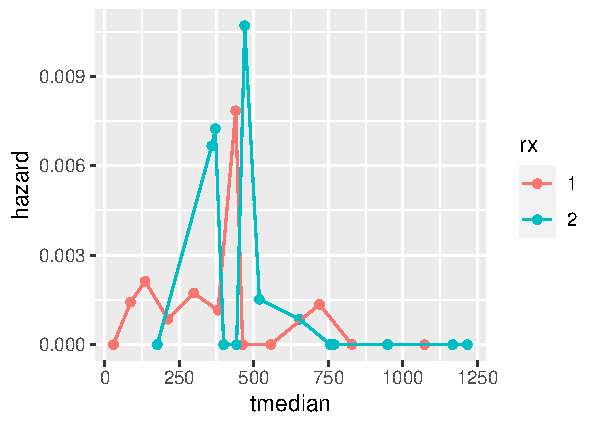
\includegraphics{Problem3_files/figure-latex/unnamed-chunk-4-1} \end{center}

\hypertarget{plot-k-m-survival-function-by-rx}{%
\section{Plot K-M survival function by
rx}\label{plot-k-m-survival-function-by-rx}}

\begin{Shaded}
\begin{Highlighting}[]
\NormalTok{ovarian.survfit }\OtherTok{\textless{}{-}}
  \FunctionTok{survfit}\NormalTok{(}\FunctionTok{Surv}\NormalTok{(futime, fustat)}\SpecialCharTok{\textasciitilde{}}\NormalTok{rx,}\AttributeTok{data=}\NormalTok{ ovarian)}

\NormalTok{ovarian.survfit }\SpecialCharTok{|\textgreater{}}
  \FunctionTok{autoplot}\NormalTok{() }\SpecialCharTok{+}
  \FunctionTok{ylab}\NormalTok{(}\StringTok{"S(t)"}\NormalTok{) }\SpecialCharTok{+}
  \FunctionTok{xlab}\NormalTok{(}\StringTok{"Time"}\NormalTok{)}
\end{Highlighting}
\end{Shaded}

\begin{center}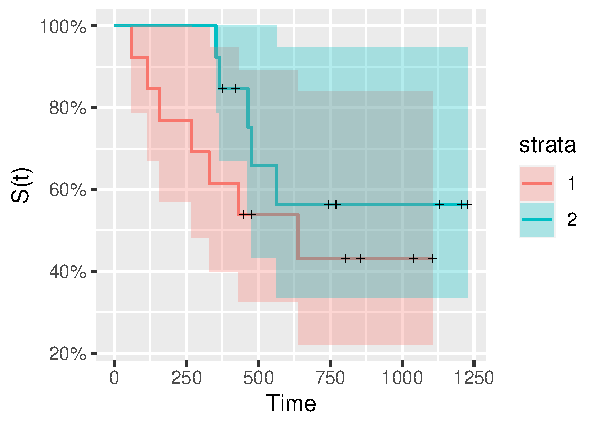
\includegraphics{Problem3_files/figure-latex/unnamed-chunk-5-1} \end{center}

\hypertarget{median-survival-time-for-each-treatment-group}{%
\section{Median survival time for each treatment
group}\label{median-survival-time-for-each-treatment-group}}

For the group 1(rx = 1), the median survival time is
\(534.5(\frac{431+638}{2})\) days. For the group 2(rx = 2), the median
survival time is not sure, because over half of patients are still
censored.

\hypertarget{compare-survival-function-estimations-between-k-m-and-f-h-methods}{%
\section{Compare survival function estimations between K-M and F-H
methods}\label{compare-survival-function-estimations-between-k-m-and-f-h-methods}}

\hypertarget{nelson-aalenfleming-harrington-and-k-m-estimators}{%
\paragraph{Nelson-Aalen(Fleming-Harrington) and K-M
estimators}\label{nelson-aalenfleming-harrington-and-k-m-estimators}}

\begin{itemize}
\tightlist
\item
  Survival function:
\end{itemize}

\[\begin
\chi_{\mathbb{Q}}(x)=
    \begin{cases}
        1 & \text{if } x \in \mathbb{Q}\\
        0 & \text{if } x \in \mathbb{R}\setminus\mathbb{Q}
    \end{cases}
\end\]

\hypertarget{descrbe-the-analyses-and-write-conclusions}{%
\section{Descrbe the analyses and write
conclusions}\label{descrbe-the-analyses-and-write-conclusions}}

\hypertarget{references}{%
\section{References}\label{references}}

Edmonson JH, Fleming TR, Decker DG, Malkasian GD, Jorgensen EO,
Jefferies JA, Webb MJ, Kvols LK. Different chemotherapeutic
sensitivities and host factors affecting prognosis in advanced ovarian
carcinoma versus minimal residual disease. Cancer Treat Rep.~1979
Feb;63(2):241-7. PMID: 445503.

\end{document}
